El sistema de archivos conforma el componente más trabajado de este núcleo. Como
ya fue explicado, elegí implementar el sistema de archivos MinixFS V2. A
continuación daré una explicación a grandes razgos de todos las características
de este FS (la mayor parte de este explicación esta basada en el libro de
Tanenbaum REFERENCIAAA, capítulo 5)

Comenzaré contando un poco la organización y distribución de la información en
minix, el superblock y manejo de blockes, poniendo la mayor atención en la idea
de inodos. A partir de ahora llamaré a el sistema de archivos MinixFS v2 como
mfs.

Doy por sabido que el lector maneja conceptos básicos de computación a bajo
nivel, por ejemplo saber que es un bloque o un mapa de bits.

\subsection{Organización en MinixFS}

Todos los sistemas de archivos modernos presentan una idea de organización de la
información, acompañada con la forma en que se guardan en el disco las
estructuras y datos necesarios para mantener esta idea. En el caso de mfs se
cuentan con una serie de estructuras que dan atributos y parametros del mismo,
seguido por el espacio vacio donde se guardan los datos en sí. La estructura
esta compuesta por: Boot Sector, Super Block, Inode Map, Zone Map, Inodes y Empty
Blocks. Esta distribución se puede apreciar en la siguiente imagen:

\begin{center}
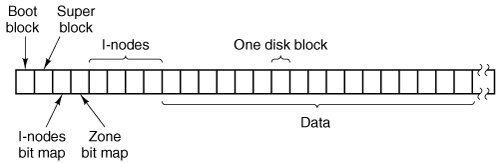
\includegraphics[scale=0.5]{../img/layout.png}
\end{center}

El Boot Sector o bs es un bloque de tamaño fijo (1024 bytes) que se encuentra
obligatoriamente al comienzo de la imagen de mfs. El uso de este bloque es una
convensión en la computación para comenzar el booteo del sistema, es el punto de
partida de la ejecución luego de que la BIOS termina la inicialización. Es por
esto que este bloque no es de mayor importancia para nosotros, simplemente hay
que tenerlo en cuenta a la hora de calcular offsets para el resto de los
bloques.

El Super Block o sb, que al igual que el bs ocupa exactamente un bloque de
tamaño fijo (1024 bytes). Mfs, al igual que todo el resto de los sistemas de
archivos, tiene una serie de atributos que pueden variar dependiendo
de las necesidades del administrador del sistema (por ejemplo el tamaño de los
bloques). Todos estos valores se encuentran en el sb, incluyendo información
necesaria como la cantidad de bloques o inodos, el tamaño máximo de un archivo,
etc. Se verá con más detenimiento es la sección correspondiente.

El Inode Map o im y Zone Map o zm. Estos dos mapas de bits son usados por mfs
para marcar cuales de las posiciones de memoria reservadas para inodos y para
datos estan usadas, im para inodos y zm para datos. En MinixFS se
hace una distinción entre Zone o zona y Block o bloque, donde una zona es un
conjunto de bloques (una potencia de dos, por ejemplo cada zona puede tener 4
bloques). La razón por la que utilizaron esta diferenciación será explicada más
adelante, pero para el trabajo que estamos haciendo esta diferencia fue evitada
asegurandose de que las zonas contengan un solo bloque.

La parte siguiente es la más importante del sistema, y corresponde al espacio de
memoria reservado para los inodos. En la sección correspondiente se explicará su
funcionamiento, pero anticipando, todo archivo esta descripto por un inodo
(aunque puede ser más de uno) que da algunas características del mismo, y una
forma de ubicar los bloques con sus datos.

Por último se encuentra la parte más grande de la imagen mfs que corresponde a
todos los bloques restantes, libres para guardar información. Por lo general
conforman el contenido de los archivos en varios bloques distribuidos por el
espacio libre, aunque en algunos casos particulares tienen información de mfs
(ver el funcionamiento de los directorios).

\subsection{Super Block}

El Supero Block o sb contiene toda la información sobre las características de
una imagen mfs en un bloque de tamaño 1024 bytes. En la siguiente imagen vemos
la distribución de la información en el bloque:

\begin{center}
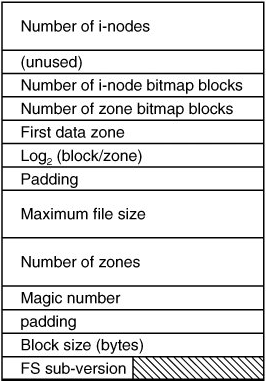
\includegraphics[scale=0.7]{../img/superblock.png}
\end{center}

La mayoría de los campos son suficientemente descriptivos como para explicarlos,
basta con afirmar que los únicos que no utilizamos son "FS sub-version" que no
juega ningun papel en la versión 2 de mfs, y "$Log_2 (block/zone)$" ya que no
hacemos distinciones entre zonas y bloques (este valore debe ser 0).

Todo el código de manejo del sb se encuentra en los archivos fs/super.c y
fs/super.h.

La primera función que debe ser llamada antes de poder interactuar con el sb es
read\_super(), que se encarga de leer el Super Block. En nuestro caso nos basta
únicamente con apuntar al inicio del sb en la memoria, ya que como explicamos
anteriormente toda la imagen mfs ya esta cargada en memoria. La estructura
superblock\_s representa al sb con los tamaños exactos como aparece en la
imagen, por lo que un puntero de este tipo nos ahorra toda necesidad de tener
que reservar espacio para la estructura y copiar los datos en la misma.

Luego la manera de interactuar con el sb es mediante defines. Una serie de
definiciones en el super.h acceden a la estructura superblock\_s para devolver
los datos. Una forma más "correcta" de hacer esto hubiese sido utilizar getters
y setters, asegurandonos en cada uno que el puntero al sb ya se hubiese
inicializado. La razón por la que no elegí este método es que read\_super() es
un método obligatorio para cualquier implementación de mfs y en caso de error la
implementación no podría seguir, por lo que es seguro asumir que no existe este
error y obviarlo. De esta manera nos ahorramos el overhead de las llamadas a los
getters y setters y trabajamos directamente con los punteros. Un ejemplo es:

\begin{verbatim}
#define IMAP_BLOCKS (sb->s_imap_blocks)
\end{verbatim}

Con 'sb' el putero a estructura superblock\_s. Este define recupera la cantidad
de bloques que ocupa el mapa de inodos.

\subsection{Inode y Zone Maps}

El mapa de inodos se encarga de mantener un registro de cuales de los espacios
reservados para inodos se encuentran ocupados. El mapa de zonas provee la misma
funcionalidad pero a nivel de bloques. Ambos son bitmaps en los cuales cada
posición posible de guardar un inodo/bloque está representado por un bit, 0 si
se encuentra libre y 1 en caso contrario.

El código para el manejo de estos mapas se encuentra también en los archivos
fs/super.c y fs/super.h.

En el caso del mapa de inodos hay 2 funciones lo manejan: rm\_inode() y
empty\_inode(). La primera se encarga de liberar la posición del inodo
asigandole un 0 al bit correspondiente. La segunda devuelve una posición libre
para crear un nuevo inodo. Logra esto manteniendo siempre un puntero a la última
posición libre del bitmap, y luego recorriendo el mapa hasta encontrar un bit
vacío.

Para el mapa de bloques existen 2 funciones similares: rm\_block() y
empty\_block(). Estas funciones se comportan de manera similar a las de inodos,
por lo que en realidad ambas son wrappers que llaman a un par de funciones
genericas free\_bit() y alloc\_bit() que son las que realizan el trabajo
descripto.

La función alloc\_bit() que encuentra un bit vacío en el bitmap es parecida a
una en el código de minix con el mismo nombre. Ambas usan una técnica simple
para rastrear ese 0 en el mapa. Recorren el bitmap de a palabras, y las comparan
con la palabra de todos 1's, logrando leer de a 32 bits por repetición del
ciclo. Al encontrar una palabra que es distinta a la completa por 1 solo hace
falta hubicar el 0 que sabemos existe.

\subsection{Inodes}

La parte más interesante de un sistema de archivos tipo Unix como lo es mfs es
la idea de inodos. Básicamente todo archivo (y como archivo contemplamos también
a directorios/pipes/links/etc.) es representado por un inodo. Un inodo esta
compuesto por una serie de campos que definen el archivo, y luego referencias a
los bloques en donde se encuentran sus datos, en el caso de tenerlos.

La función principal de un inodo es referenciar todos los bloques que conforman
un archivo. Lo bueno de este método es que al abrir y leer un archivo, solo es
necesario mirar a su inodo, éste tiene toda la información necesaria para
leerlo. Esto es una mejora substancial comparado con sistemas del tipo FAT, que
requieren de una tabla aparte con la información de todos los archivos. En este
último caso una tabla de este estilo sería enorme para los tamaños de los discos
en la actualidad, y ocuparia varios Mbyes en memoria constantemente. En cambio
con inodos solo es necesario mantener en memoria aquellos que se encuentran
actualmente en uso, aprovechando mejor los recursos.

A continuación se muestra un gráfico con la estructura general de un inodo en
mfs (similar a los inodos en ext2 o cualquier otro fs tipo unix):

\begin{center}
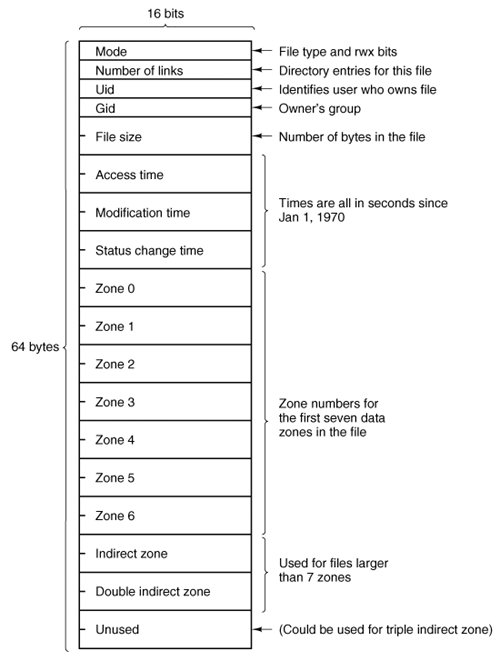
\includegraphics[scale=0.5]{../img/inode.png}
\end{center}

Esta imagen (al igual que el resto de las utilizadas en esta sección MinixFS)
fue tomada del libro de Tanembaum REFERENCIA, y contiene descripciones de los
campos que conforman el inodo: 'mode' que nos da el tipo de archivo y sus
atributos de lectura/escritura/ejecución; 'links' nos dice cuantos directorios
contienen al archivo (es decir cuantos 'hard links' existen); 'uid/gid' el dueño
y su grupo; 'size' el tamaño; 'access/mod/status time' tiempos varios; 'zone
0-6' los punteros a los primeros 7 bloques del archivo.

Paramos aquí para comentar una característica de los inodos. Para poder contar
con archivos suficientemente grandes, se implemento la idea de bloques
indirectos/doble indirectos/triple indirectos. En caso de que la
información del archivo supere el espacio que proveen los primeros 7 bloques
referenciados en el inodo, se pasa al bloque de indirectos, que consta de un
bloque completo con punteros a otros bloques donde sigue el archivo. En caso de
que éste último no alcanze, se repite la idea y se utiliza el doble indirecto,
que apunta a un bloque con punteros a otros bloques, que a su vez contienen
punteros a bloques con la información. Para entender mejor el funcionamiento ver
el siguiente gráfico:

\begin{center}

\includegraphics[scale=0.5]{../img/inode_links.png}
\end{center}

De esta manera se logra expandir el limite del tamaño de un archivo los
suficiente como para que no sea un problema. En el caso de mfs los bloques
triple indirectos no son utilizados, pero el espacio en el inodo existe por si
fueran a ser necesarios en el futuro.

Veamos ahora como se implementan en nuestro sistema. El código de manejo de
inodos se encuentra en los archivos fs/inode.c y fs/inode.h, con partes menores
en fs/fs.c.

La función más interesante en el manejo de inodos es find\_inode(), que dado un
directorio de inicio y un path tipo unix (ej. jp/orga2/informe.pdf), encuentra y
devuelve el inodo buscado en caso de existir (en nuestro ejemplo sería el inodo
correspondiente al archivo informe.pdf). La implementación permite que se pueda
borrar el archivo en cuestion, se cree, o simplemente que se devuelva. Por
ejemplo, para conseguir el inodo correspondiente al archivo '/home/jp/hola.txt',
bastaría con llamar a la la función find\_inode(NULL, "/home/jp/hola.txt",
FS\_SEARCH\_GET).

Luego de decidir por donde empezar la busqueda (si el path empieza con '/'
empezamos en el root directory), esta función se encarga de ir componente por
componente navegando los directorios del path y avanzando hasta el último
subdirectorio. Logra esto utilizando la función search\_inode(), que dado un
directorio y un nombre de archivo, devuelve el numero inodo correspondiente, en
caso de que exista.

Analicemos más de cerca esta última función. Comienza recorriendo un
directorio entrada por entrada buscando aquella que coincide con el nombre de
archivo/carpeta buscado. Hace uso de varias funciones auxiliares que
detallaremos a continuación. El siguiente extracto de código de search\_inode()
muestra el loop principal:

\begin{verbatim}
for (pos = 0; pos < dir->i_size; pos += BLOCK_SIZE) {
    /* get the block with the files/subdirectories */
    dentry = (struct dir_entry_s *) get_block(read_map(dir, pos));
    end = dentry + NR_DIR_ENTRIES;

    /* cycle through the dir entries and search for the required name */
    for (; dentry < end; dentry++) {
        if (empty == NULL && dentry->num == 0)
            empty = dentry;
        if (dentry->num != 0 && mystrncmp(name, dentry->name, MAX_NAME) == 0)
            return dentry;
    }
}

return empty;
\end{verbatim}

La manera en que el código recorre las entradas del directorio es mediante la
función read\_map(), que dado una posición de un archivo/carpeta, devuelve el
bloque en que se encuentra (es decir, resuelve bloques
directos/indirectos/etc.); get\_block() simplemente devuelve
un puntero al inicio del bloque pedido. Así vamos bloque por bloque recorriendo
todas las entradas del directorio, comparando una por una con la función
mystrncmp (una imitación de strncmp de la biblioteca estandar, recordar que no
contamos con ninguna de estas funciones). En el caso de que no se encuentre la
entrada que se buscaba, search\_inode() devuelve una entrada vacía. Esto es muy
util para implementar llamadas como rename(), pudiendo agregar un archivo a un
directorio.

Es importante aclarar que hay una diferencia clave con la manera en que está
implementado mfs en minix. Funciones como get\_block() requieren llamar al
disco, recobrar el bloque en cuestión y guardarlo en memoria para poder
utilizarlo. En cambio nosotros simplemente apuntamos a la posición de dicho
bloque, ya que todo se encuentra pre-cargado. Lo mismo sucede con los inodos y
la función get\_inode(), en la implementación real del fs se mantiene una cache
de inodos que contiene todos aquellos que se están utilizando en ese momento,
lo cual no es necesario en nuestro caso por el mismo motivo.

\subsection{System Calls del FS}

Los sistemas tipo unix utilizan la idea de descriptor de archivo o 'fd' para
identificar archivos abiertos. Cuando un programa quiere abrir un archivo, se le
es entregado este fd, que no es más que un número identificador. Luego basta
utilizar este número para realizar cualquier acción sobre el archivo
(leer/escribir/etc.).

Las funciones de manipulación de fds se encuentran en los archivos fs/file.c y
fs/file.h. Cada proceso en su tabla contiene un arreglo con los fds y
sus respectivos inodos. Mediante las funciones get\_fd() y release\_fd(), uno
reserva y devuelve fds según las necesidades del proceso.

La implementación de estas funciones hace uso de el archivo sys/queue.h, una
implementación estándar de listas para los sistemas unix. Declarando un par de
punteros en el arreglo de fds, simulamos una lista tipo fifo con la que nos
aseguramos que pedir y devolver fds sea siempre $O(1)$. En el caso de get\_fd()
tenemos:

\begin{verbatim}
int get_fd(ino_t ino_num, unsigned int pos)
{
    struct file_s *file = LIST_FIRST(&unused_fd);

    if (file != NULL) {
        LIST_REMOVE(file, unused);
        file->ino = ino_num;
        file->pos = pos;
        return file->fd;
    }

    return ERROR;
}
\end{verbatim}

De esta manera podemos utilizar la idea de listas sin tener que agregar
complicaciones al código, y más que nada no tenemos que introducir memoria
dinámica, ya que los arreglos que simulan la lista son estáticos y por ende
fijos.

Con el manejo de fds completo, comienza el código que rearma todo lo ya
explicado para implementar las llamadas al sistema. Para cada system call unix,
la función que la recibe tiene el prefijo "sys\_" (por ejemplo, la función
sys\_open() atiende la llamada open()). Se implementaron las llamadas open(),
close(), write(), read(), lseek(), unlink() y rename() para manejo de archivos,
chdir(), mkdir(), rmdir() y getdents() para manejo de carpetas.

Las implementación de estas funciones se encuentra en los archivos fs/fs.c y
fs/fs.h. Veamos como se hicieron algunas de estas funciones.

En el caso de read() y write(), comenzaron siendo funciones distintas, pero
rápidamente me di cuenta que el código entre ellas era muy similar, por lo que
decidí separarlo en la función fs\_readwrite(). Esta se encarga de leer o
escribir un archivo, dependiendo de la flag que se le provee.

\begin{verbatim}
while (n > 0) {
    if ( (blocknr = read_map(ino, pos)) == NO_BLOCK)
        return ERROR;
    block = (char *) get_block(blocknr);

    off = pos % BLOCK_SIZE;
    size = MIN(n, BLOCK_SIZE - off);

    if (flag == FS_WRITE)
        mymemcpy(block + off, buf, size);
    else
        mymemcpy(buf, block + off, size);

    n -= size;
    pos += size;
    buf += size;
}
\end{verbatim}

El loop principal de fs\_readwrite() va navegando los bloques del archivo con
read\_map() y, dependiendo si se busca leer o escribir, utiliza la función
mymemcpy para realizar el trabajo (que es un clon de la función de mismo nombre
de la biblioteca estándar).

El resto de las llamadas de archivo son simples, open() y close() solo manejan
fds con las funciones antes descriptas; unlink() llama a find\_inode() pidiendo
que se borre el archivo; rename() busca ambos paths y intercambia la entrada;
lseek() modifica el puntero al archivo en la lista de fds.

Por el lado de manejo de directorios, rmdir() remueve un directorio asegurandose
primero que este vacío; chdir() cambia el directorio actual (el inodo del
directorio actual se guarda en la tabla del proceso); mkdir() crea un directorio
mediante find\_inode(). 
